\documentclass[a4paper,10pt]{article}
%\documentclass[a4paper,10pt]{scrartcl}

\usepackage[utf8]{inputenc}
\usepackage[T1]{fontenc}
\usepackage{graphicx}
\usepackage{etoolbox}
\usepackage[hidelinks]{hyperref}
\usepackage{geometry}
\usepackage[parfill]{parskip}
\usepackage{xcolor}

\usepackage{fancyhdr}
\pagestyle{fancy}
\setlength{\footskip}{35mm}
\lhead{}
\lfoot{\textit{\textcolor{gray}{Adam Dobbs}}}
\cfoot{\textit{\textcolor{gray}{The MAUS Workbook}}}
\rfoot{\textit{\textcolor{gray}{ver. 1.9}}}

\usepackage{listings}
\lstdefinestyle{customcpp}{
  belowcaptionskip=1\baselineskip,
  breaklines=true,
  %frame=L,
  xleftmargin=\parindent,
  language=C++,
  showstringspaces=false,
  basicstyle=\ttfamily,
  keywordstyle=\bfseries\color{green!40!black},
  commentstyle=\color{gray},
  identifierstyle=\color{black},
  stringstyle=\color{red},
}
\lstdefinestyle{custompy}{
  belowcaptionskip=1\baselineskip,
  breaklines=true,
  %frame=L,
  xleftmargin=\parindent,
  language=Python,
  showstringspaces=false,
  basicstyle=\ttfamily,
  keywordstyle=\bfseries\color{green!40!black},
  commentstyle=\color{gray},
  identifierstyle=\color{black},
  stringstyle=\color{red},
}
\lstdefinestyle{custombash} {
  language=Bash,
  basicstyle=\ttfamily,
  keywordstyle=\color{black},
}
\lstdefinestyle{custommake} {
  belowcaptionskip=1\baselineskip,
  breaklines=true,
  %frame=L,
  xleftmargin=\parindent,
  language=make,
  showstringspaces=false,
  basicstyle=\ttfamily,
  keywordstyle=\bfseries\color{green!40!black},
  commentstyle=\color{gray},
  identifierstyle=\color{black},
  stringstyle=\color{red},
}

\lstset{style=custompy}


\renewcommand{\familydefault}{\sfdefault}

\makeatletter
\patchcmd{\@maketitle}{\LARGE}{\fontsize{45}{3}\selectfont}{}{}
\makeatother

\title{\textcolor{blue}{The MAUS Work Book}}
\author{Adam Dobbs}
\date{Version 2.0, May 2016}

% \pdfinfo{%
%   /Title    (MAUS Work Book)
%   /Author   (Adam Dobbs)
%   /Creator  (Adam Dobbs)
%   /Producer (Adam Dobbs)
%   /Subject  (MAUS)
%   /Keywords (MAUS)
% }

\begin{document}

\thispagestyle{empty}

\vspace*{1cm}

{\let\newpage\relax\maketitle}

\reversemarginpar

\thispagestyle{empty}
\vspace{2cm}

\begin{figure}[h]
 \begin{center}
   
\includegraphics[width=0.29\linewidth]{./graphics/mice-logo.pdf}
 \end{center}
\end{figure}

\vspace{5cm}

\pagebreak

\tableofcontents

\pagebreak

\section{Glossary of Terms}
\begin{itemize}
  \item \textbf{ADC} - Analogue-to-Digital Converter
  \item \textbf{API} - Application Programme Interface
  \item \textbf{BASH} - Bourne Again Shell, a linux command line programme
  \item \textbf{Bazaar} - A distributed version control system
  \item \textbf{CKOV} - Threshold cherenkov detectors
  \item \textbf{Datacard} - A list of variables passed into MAUS (actually a Python script)
  \item \textbf{DAQ} - Data Aquisition system
  \item \textbf{EMR} - Electron Muon Ranger, a calorimeter
  \item \textbf{KL} - KLOE-Lite detector
  \item \textbf{GEANT4} - Framework to simulate passage of particles through matter
  \item \textbf{GRID} - A network of computing resources used for large scale data processing
  \item \textbf{JSON} - Jave Script Object Notation, an ASCII format
  \item \textbf{MAUS} - MICE Analysis User Software
  \item \textbf{MICE} - Muon Ionization Cooling Experiment
  \item \textbf{MC} - Monte Carlo simulation
  \item \textbf{PID} - Particle Identification
  \item \textbf{ROOT} - The standard high energy physics analysis framework, see \url{https://root.cern.ch}
  \item \textbf{Spill} - Data class in MAUS, corresponds to the data produced in MICE for one dip of the pion production target
  \item \textbf{TDC} - Time-to-Digital Converter
  \item \textbf{TOF} - Time of Flight, or the associated detectors
  \item \textbf{Tracker} - Scintillating fibre trackers
  \item \textbf{UI} - User Interface
  \item \textbf{Unpacker} - A third party library bundled with MAUS, used internally to extract data from the MAUS DAQ binary format
\end{itemize}

\pagebreak

\section{MAUS Description}
\label{sec:MAUSDescription}
  MAUS stands for MICE Analysis User Software. MICE itself refers to the Muon Ionization Cooling experiment, see the website for more details:

  \medskip
  \url{http://www.mice.iit.edu}. % \marginpar{\textcolor{cyan}{MICE\linebreak Website}}
  \medskip

  MAUS is the official software framework for the simulation and reconstruction of the MICE data. It also provides an environment which can be used for developing subsequent analysis tools, and provides the libraries neccessary for using other tools to access processed MICE data.
  
  This workbook constitutes a quick start guide for MAUS.  It covers the following standard tasks:
  
  \begin{itemize}
    \item Performing simulations;
    \item Unpacking and reconstructing raw MICE data;
    \item Accessing and analysing simulated and reconstructed data.
  \end{itemize}

  A much fuller description of MAUS can be found in the User Guide, available at:

  \medskip
  \url{http://micewww.pp.rl.ac.uk/maus/MAUS_latest_version/maus_user_guide/index.html}. % \marginpar{\textcolor{cyan}{User Guide}}

\section{Installing MAUS}
\label{sec:InstallingMAUS}
  This section provides a summary of how to install MAUS on a Linux operating system. MAUS officially supports Scientific Linux 6 and recent versions of CentOS only, however unofficially MAUS should compile on many modern linux distributions, including Ubuntu.  A more detailed guide to installing MAUS, including a list of prerequisites, can be found on the MAUS wiki:

  \url{http://micewww.pp.rl.ac.uk/projects/maus/wiki/Install}

  \subsection{Obtaining the Code}
    MAUS may be obtained in one of two ways. First, MAUS releases are available for download as gzipped tarballs from:

    \medskip
    \url{http://micewww.pp.rl.ac.uk/maus/} 
    \medskip

    Alternatively MAUS may be branched using the Bazaar distributed version control system (see \url{http://bazaar.canonical.com}) from the Launchpad code hosting website. The MAUS page on Launchpad is \url{https://launchpad.net/maus}. A detailed guide to using Bazaar with MAUS can be found on the MAUS wiki at \url{http://micewww.pp.rl.ac.uk/projects/maus/wiki/Bzr_usage} (see section~\ref{sec:UsefulInformation}). In order to branch the latest release use:
    \begin{lstlisting}
bzr branch lp:maus
    \end{lstlisting}
    In order to obtain the latest development code (not for use if doing analyses) use:
    \begin{lstlisting}
bzr branch lp:maus/merge
    \end{lstlisting}

  \subsection{Installation}
    Once the MAUS source code has been obtained, move into the source root directory. Inside this directory is a BASH script named \texttt{install\_build\_test.sh}. Execute this script to perform the full MAUS installation. On multicore machines use the flag ``\texttt{-j N}'' where \texttt{N} is the number of processor threads to use. For example, to install with two threads:
    \begin{lstlisting}
./install_build_test.sh -j 2
    \end{lstlisting}
    If another fully built MAUS installation of the same release is already present on the system, then the third party libraries from that installation can be linked against instead of building them from scratch (saving a lot of disk space and time during installation).  This is done by specifying the location of the other MAUS installation with a ``\texttt{-t}'' flag, for example:
    \begin{lstlisting}
./install_build_test.sh -t /path/to/other/maus
    \end{lstlisting}

  \subsection{Preparing to run}
    Prior to running, the MAUS envionment variables must be loaded into the local shell environment each time a new shell is used.  This is done by sourcing the script ``env.sh'' found in the MAUS root directory:
    \begin{lstlisting}
source env.sh
    \end{lstlisting}
    \textbf{\textcolor{blue}{MAUS is now ready to use!}}
    
  \subsection{Rebuilding}
  If any code within MAUS is modified, it will need to be rebuilt for the changes to take effect. MAUS uses the \textit{scons} build system (a Make replacement based on Python). To rebuild MAUS, simply type \texttt{scons} from the MAUS root directory (after sourcing the environment). A flag \texttt{-jN} may also be supplied to run on multiple threads. In order to clean the build before rebuilding, the command \texttt{scons -c} may be used.
  
  \subsection{Choosing the Unpacker}
  The unpacker is a third party library which ships with MAUS, and is used internally for extracting the raw binary data produced by the MICE DAQ. There are two versions of the unpacker present in MAUS, one corresponding to MICE Step I data, the other to MICE Step IV and later data. From MAUS release 0.9.5 the default unpacker is set to be Step IV.

  To switch between unpackers, a simple utility script, \texttt{switch\_unpacker.bash}, is provided in the MAUS root directory. To switch unpackers, source the MAUS environment and then source (not run) this script, supplying an argument of either of StepI or StepIV. This will edit \texttt{env.sh}, change the \texttt{MICE\_ UNPACKER\_VERSION} environment variable, rebuild the unpacker, and clean and rebuild MAUS.

  \textbf{NB}: The \texttt{switch\_unpacker.bash} script only works for full MAUS installations; if the MAUS installation links against third parties from another installation, the script will abort.  In this case, change the unpacker version in the full MAUS installation first using the script, then in the linked MAUS installation edit env.sh so that \texttt{MICE\_ UNPACKER\_VERSION} is set to the correct value, and clean and rebuild MAUS manually.

\section{An Introduction to the MAUS UI and API}
\label{sec:API}
  \subsection{The API}
    MAUS is written in both C++ and Python, with Python primarily in the code presented to the user, and C++ primarily in the backend to do the hard work.  MAUS is split up into different modules which can be chained together to perform various tasks. Data is passed between each module via an instance of a class known simply as \textit{Data}. Within the Data object the rest of the MAUS data structure is nested (see section~\ref{sec:Datastructure}). 

    There are four types of module present in MAUS:
    \begin{itemize}
      \item \textbf{Input} - modules which read in data, such as from the DAQ or a ROOT file
      \item \textbf{Map} - modules which perform most of the work of simulation and reconstruction
      \item \textbf{Reduce} - modules which accumulate data in order to produce plots
      \item \textbf{Output} - writes out processed data to e.g. a ROOT or JSON file 
    \end{itemize}
    \noindent
    Modules are chained together using a Python script to create a functional MAUS programme.  This is illustrated in figure~\ref{fig:MapReduce}.
    
    \begin{figure}[h]
      \begin{center}
        
\includegraphics[width=0.8\linewidth]{./graphics/map-reduce.pdf}
        \caption{The MAUS Map - Reduce scheme.}
        \label{fig:MapReduce}
      \end{center}
    \end{figure}

  \subsection{Creating a MAUS programme}
    All the core MAUS modules and classes may be imported into Python ready for use by using the command:
\lstset{language=Python} 
    \begin{lstlisting}
import MAUS
    \end{lstlisting}
    Each desired input, map, reduce and output module must then be declared.  For example, to declare an input module used to setup the spill structure ready for a simulation:
    \begin{lstlisting}
my_input = MAUS.InputPySpillGenerator()
    \end{lstlisting}
    There must only be one input and output module used.  However, multiple maps and reducers may be used by grouping them together using the special modules \texttt{MapPyGroup} and \texttt{ReducePyGroup}. For example, to group together the maps needed for a GEANT4 beam simulation:
    \begin{lstlisting}
my_map.append(MAUS.MapPyBeamMaker())   # Beam construction
my_map.append(MAUS.MapCppSimulation()) # GEANT4 simulation
    \end{lstlisting}
    Also, if no maps or reducers are required, the ``do nothing'' modules, \texttt{MAUS.MapPyDoNothing()} and \texttt{MAUS.ReducePyDoNothing()} must be used.

    After declaring all the required MAUS modules, a special class known as \texttt{datacards} for handling the passing of parameters must be declared. Datacards are collections of parameters used by MAUS, and are discussed in section~\ref{sec:RunningAProgramme}. To use only parameters passed from the command line or via a datacard, with the rest set to their default values, the following declaration is used:
    \begin{lstlisting}
datacards = io.StringIO(u"")
    \end{lstlisting}

    Finally, all the modules and datacards are passed to a special class called ``Go'', which runs each module in turn and passes the data from one to another:
    \begin{lstlisting}
MAUS.Go(my_input, my_map, my_reduce, my_output, datacards)
    \end{lstlisting}

  \subsection{A Minimal Working Example}
    A minimal working example which performs a GEANT4 beam simulation, reconstructs the Time-of-Flight (TOF) detector data and writes the output to a ROOT file is shown below:
    %\begin{lstlisting}[language=Python]
    \begin{lstlisting}
import io   # Generic Python library for I/O
import MAUS # MAUS libraries

def run():
  my_input = MAUS.InputPySpillGenerator()
  my_map = MAUS.MapPyGroup()
  my_map.append(MAUS.MapPyBeamMaker())   # Beam construction
  my_map.append(MAUS.MapCppSimulation()) # GEANT4 simulation
  my_map.append(MAUS.MapPyMCReconSetup()) # Detector setup
  my_map.append(MAUS.MapCppTOFMCDigitizer()) # TOF MC Digitizer
  my_map.append(MAUS.MapCppTOFSlabHits())    # TOF Slab Hits
  my_map.append(MAUS.MapCppTOFSpacePoints()) # TOF Spacepoints
  my_reduce = MAUS.ReducePyDoNothing()
  my_output = MAUS.OutputCppRoot()
  datacards = io.StringIO(u"")
  MAUS.Go(my_input, my_map, MAUS.ReducePyDoNothing() \
          my_output, datacards)

if __name__ == '__main__':
    run() 
    \end{lstlisting}

\lstset{style=custombash}

  \subsection{Running a MAUS Programme and Using Datacards}
  \label{sec:RunningAProgramme}
    Once the Python script has been created it can be executed using the Python interpreter (remembering to \texttt{source env.sh} first). For example to run a script called ``my\_programme.py'' use:
   \begin{lstlisting}
python my_programme.py
    \end{lstlisting}
    
    It is also important to consider what parameter values the programme requires.  MAUS uses a large set of parameters to configure how it runs, covering areas such simulation beam parameters, input and output file names, which geometry files to use, etc.  The default values for all these parameters are set in the file \texttt{src/common\_py/ConfigurationDefaults.py}. Parameters may be modified from their default values in one of three ways. 
    
    \begin{enumerate}
     \item By passing arguments to the executable Python script.  The required syntax is \texttt{-{}-variable-name value}. For example to change the name of the output ROOT file from its default value of ``maus\_output.root'' to ``my\_output.root'' when running a programme defined by the Python script \texttt{my\_programme.py}, the following command could be used:
     \begin{lstlisting}
python my_programme.py --output_root_file_name my_output.root
    \end{lstlisting}
    \item With a datacards file. A datacards file is simply a list of parameters and values, one per line, of the form:
    \begin{lstlisting}
variable=value
    \end{lstlisting}
    A datacard may be passed to an executable by using the \texttt{-{}-configuration\_file} flag. For example, to run a script called ``my\_programme.py'' together with a datacard called ``datacard.py'':
    \begin{lstlisting}
python my_programme.py --configuration_file datacard.py
    \end{lstlisting}
    \item From within the executable Python script. By modifying the line
    \begin{lstlisting}
datacards = io.StringIO(u"")
    \end{lstlisting}
    parameters may be set by assigning them a value between the speech marks.
    \end{enumerate}
    Generally, if only one or two parameters require setting, method~1 is easiest, otherwise use method~2. 

    \textbf{NB}: Only use one method at a time, or some of the settings may be ignored! Some parameters and their default values are listed in appendix~\ref{sec:CommonParameters}.

\section{The Datastructure}
\label{sec:Datastructure}

MAUS uses a large and complex data structure to store all the MC simulation, raw detector and reconstruction data.  A diagram illustrating the data structure can be found at:

\url{http://micewww.pp.rl.ac.uk/maus/MAUS_latest_version/maus_user_guide/node10.html}

Perhaps more helpfully, the data structure is extensively documented using the Doxygen documentation system, available at:

\url{http://micewww.pp.rl.ac.uk/maus/MAUS_latest_version/doc/index.html}

The top level object in the data structure is a class called simply \textit{Data}. This contains run and job header and footer information (such as the version of MAUS used, the date of the run, etc) together with a single \textit{Spill} object. A Spill represents all the experimental data associated with one dip of the MICE pion production target; all MC, raw detector and reconstruction data is contained within it.

The Spill is split into three main branches: 

\begin{itemize}
  \item \textit{MCEvent} holds the MC truth data for every track together with all MC detector and virtual hits produced;
  \item \textit{DAQData} holds the raw, unpacked data for each detector (such as ADC and TDC values)
  \item and \textit{ReconEvent} holds the reconstructed data for each detector.
\end{itemize}

Examples showing how to access and navigate the data structure for analysis are given in section~\ref{sec:Analysis}.

\section{Geometry}
\label{sec:Geometry}
MAUS uses a sophisticated GDML-based geometry for use in both simulation and reconstruction (by default the same geometry is used for both).  The canonical geometry is stored in the MICE configuration database (CDB), while an older legacy geometry is stored locally in MAUS (currently still the default option).

The CDB is a bitemporal database, that is it stores geometry configurations based on upload date and date of validity.  A particular CDB geometry must be downloaded to the local MAUS installation before it may be used by a programme.  This can be done using a utility script, \texttt{download\_geometry.py}, located in \texttt{bin/utilities}.  The script queries the CDB and then downloads the required geometry.  Geometries can be selected for download by a number of methods:

\begin{enumerate}
  \item Retrieve current geometry:
  \begin{lstlisting}
./bin/utilities/download_geometry.py
   --geometry_download_by current
  \end{lstlisting}
  \item By geometry ID  e.g. 
    \begin{lstlisting}
./bin/utilities/download_geometry.py --geometry_download_id 123
    \end{lstlisting}
  \item By run number e.g.
  \begin{lstlisting}
./bin/utilities/download_geometry.py
   --geometry_download_by run_number
   --geometry_download_run_number 6008
  \end{lstlisting}
\end{enumerate}

Additional beamline settings may also be specified, for example to download a geometry by ID for a particular beamline line mometum with all cooling channel magnet currents set to zero:

\begin{lstlisting}
./bin/utilities/download_geometry.py 
      --geometry_download_by "id" 
      --geometry_download_id 123
      --geometry_download_coolingchannel_tag  "NoField" 
      --geometry_download_beamline_tag "6-200+M0" 
\end{lstlisting}

If no beamline options are specified a 200MeV/c beamline setting with 4~T field in the cooling channel is used.

A list of the current geometries and the runs associated with them are available from:

    \medskip
    \url{http://micewww.pp.rl.ac.uk/projects/maus/wiki/GeometryDescriptions}
    \medskip

By default, downloaded CDB geometries are stored in \texttt{files/geometry/download}.  A simulation or reconstruction script can be told to use a particular geometry by using the flag \texttt{-{}-simulation\_geometry\_file} followed by the absolute path and the top level geometry file name, \texttt{ParentGeometryFile.dat}. For simulation usage examples see section~\ref{sec:Simulation}, and for reconstruction usage examples see section~\ref{sec:Reconstruction}.

\section{Running a MC Simulation}
\label{sec:Simulation}
  An example script for running a full MC simulation of MICE can be found in the bin directory:
  \begin{lstlisting}
./bin/simulate_mice.py
  \end{lstlisting}
  This will produce a ROOT output file which can be used for analysis.  

  It is generally desirable to customise the simulation in some way by passing datacard variables. For example to specify a particular geometry to use from the CDB, first download the desired geometry as described in section~\ref{sec:Geometry}. A new reference simulation particle must also then be defined (due to differences between the local legacy geometry and the CDB geometries) via a datacard parameter. This can be defined in a datacard file as:
  \begin{lstlisting}
simulation_reference_particle = {"position":{"x":0.0, "y":0.0, "z":1000.0}, "momentum":{"x":0.0, "y":0.0, "z":1.0}, "particle_id":-13, "energy":226.0, "time":0.0, "random_seed":10, "spin":{"x":0.0, "y":0.0, "z":1.0}}
  \end{lstlisting}
  This gives a reference particle starting at coordinates (0, 0, 1000) (in mm), $p_z = 1$~MeV/c, species $\mu^+$ with energy 226~MeV. If the above line is stored in a file ``datacard.py'', the new simulation can be run with:
  \begin{lstlisting}
./bin/simulate_mice.py --simulation_geometry_file /path/to/maus/files/geometry/download/ParentGeometryFile.dat --configuration_file datacard.py 
  \end{lstlisting}
  For details on the rest of the options available when performing simulations, see the full MAUS user guide.

\section{Reconstructing Real MICE Data}
\label{sec:Reconstruction}

  \subsection{Do I Need to be Reconstructing Data Myself?}
  Before reconstructing raw MICE data, it is important to stop and consider whether this is the best workflow for the task in hand. All MICE data should already be available unpacked and reprocessed from one of the standard locations listed in \ref{sec:Analysis}. This reprocessing will have been done using an official release version of MAUS with a standard set of parameters - hence \textbf{anyone thinking of analysing data for publication should use the official processed data instead of processing themselves}. If this does not dissuade you, then read on.

  \subsection{Obtaining the Raw Data}
    MICE data is recorded by MICE DAQ as custom format binary files.  This data is available for download from a web interface hosted at:

    \medskip
    \url{http://www.hep.ph.ic.ac.uk/micedata/}
    \medskip

    For those with GRID credentials who are members of the MICE virtual organisation, the data may also be obtained from the GRID at LFC location \texttt{/grid/mice/MICE/}.

    The data is distributed as tar archives. Once extracted the binary data files can be identified by their filenames, which follow the format \texttt{<run\_number>.nnn} where \texttt{nnn} is a number corresponding to the data block of the run respresented by the file, beginning at \texttt{000}.

  \subsection{Unpacking and Reconstructing}
    An example script which unpacks the binary data and reconstructs data from all the MICE dectors can be found in the bin directory.  Parameters indicating the location and name of the binary data file must be passed in, together with the appropriate geometry for the run being analysed (the desired geometry must be downloaded first, as described in section~\ref{sec:Geometry}).  For example:
    \begin{lstlisting}
python ./bin/analyze_data_offline.py \
         --daq_data_path /path/to/data/ \
         --daq_data_file file.name \
         --simulation_geometry_file /path/to/maus/files/geometry/download/ParentGeometryFile.dat
    \end{lstlisting}
    (Note we specify the simulation geometry file, as the reconstruction geometry will default to the same value.) This will produce a ROOT file containing all the unpacked raw data and the reconstrucuted data, ready for analysis.

\section{Analysing Output Data}
\label{sec:Analysis}

  \subsection{Obtaining Data for Analysis}

  \begin{figure}[tbh]
    \begin{center}
      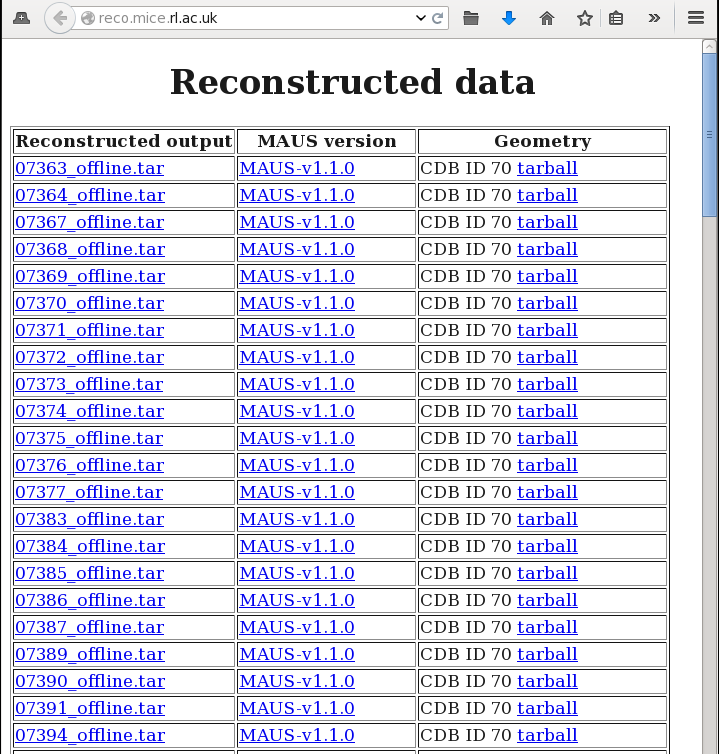
\includegraphics[width=0.34\linewidth]{./graphics/OffRecReconWebStore.png} \hspace{5mm}
      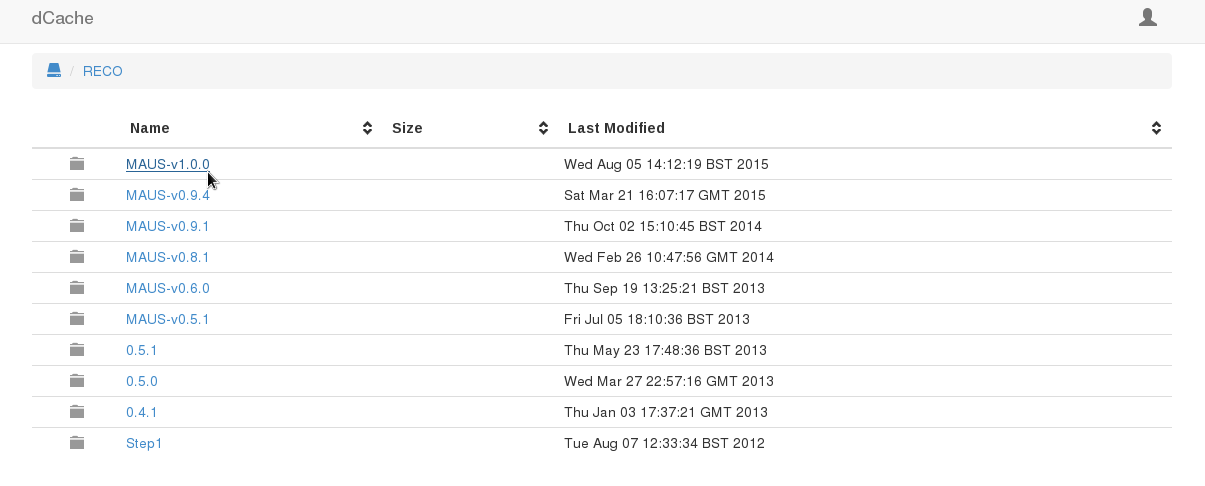
\includegraphics[width=0.6\linewidth]{./graphics/WebStoreReco.png}
      \caption{Left:The offrec machine reconstucted data page (for current processed data). Right: The GRID MICE data webstore, reconstruction section (for older processed data).}
      \label{fig:WebStoreReco}
    \end{center}
  \end{figure}

  Data from simulation may be produced by MAUS as described in section~\ref{sec:Simulation}.  For real data, as mentioned in section~\ref{sec:Reconstruction}, the preferred route is for analysts to use MICE data which has been unpacked and reconstructed centrally, either on the offical MICE offline reconstruction machines or via the GRID for older data.  This ensures everyone is using the same standard reconstruction parameters from an official release of MAUS, and is especially important if the analysed data is intended for publication. If it is still desirable to reconstruct data locally with MAUS prior to analysis, see section~\ref{sec:Reconstruction}.  Otherwise, centrally processed MICE data from the offrec machines is made available from:

  \url{http://reco.mice.rl.ac.uk/}

  Older data processed on the GRID is available from the MICE webstore:

  \url{http://www.hep.ph.ic.ac.uk/micedata/RECO/}

  The web page for the offrec machines processed data is shown in figure~\ref{fig:WebStoreReco} (left). Data is stored by ascending run number in tarball archives which may be downloaded.  Inside each tar archive there are a number of log files and parameter files. The data itself is stored in a ROOT file following the naming convention \texttt{xxxxx\_recon.root}, where \texttt{xxxxx} is the run number. Also on the page is information of the MAUS verison used to perform the reconstruction, together with a link to the geometry used.

  The front page of the reconstruction section of the GRID  webstore is shown in figure~\ref{fig:WebStoreReco} (right). The data in the webstore is organised by MAUS version used to perform the reconstruction, by parameter set used in the reconstruction (assigned a unique number known as the batch iteration number or BIN) and by run number. The data for each run is again stored in a tarball file archive.

  A catalogue of MICE runs, including run numbers, run conditions, beamline optics, number of triggers taken, etc. is available via the MICE CDB viewer:

  \url{http://cdb.mice.rl.ac.uk/cdbviewer/}

  \subsection{Understanding the ROOT file}
  By default, simulated and reconstructed data produced by MAUS is stored in a ROOT file, and data processed on the GRID is also stored in this format.  The top level object in a MAUS ROOT file is a ROOT TTree called ``Spill''. This TTree contains a branch holding a MAUS data structure Data object, which in turn contains a MAUS data structure Spill object (not to be confused with the TTree called Spill).  All the raw detector, MC and reconstruction data is found within this Spill object.  The top few levels of a MAUS ROOT file, displayed in a TBrowser, are shown in figure~\ref{fig:TBrowser}.

  \begin{figure}[tb]
    \begin{center}
      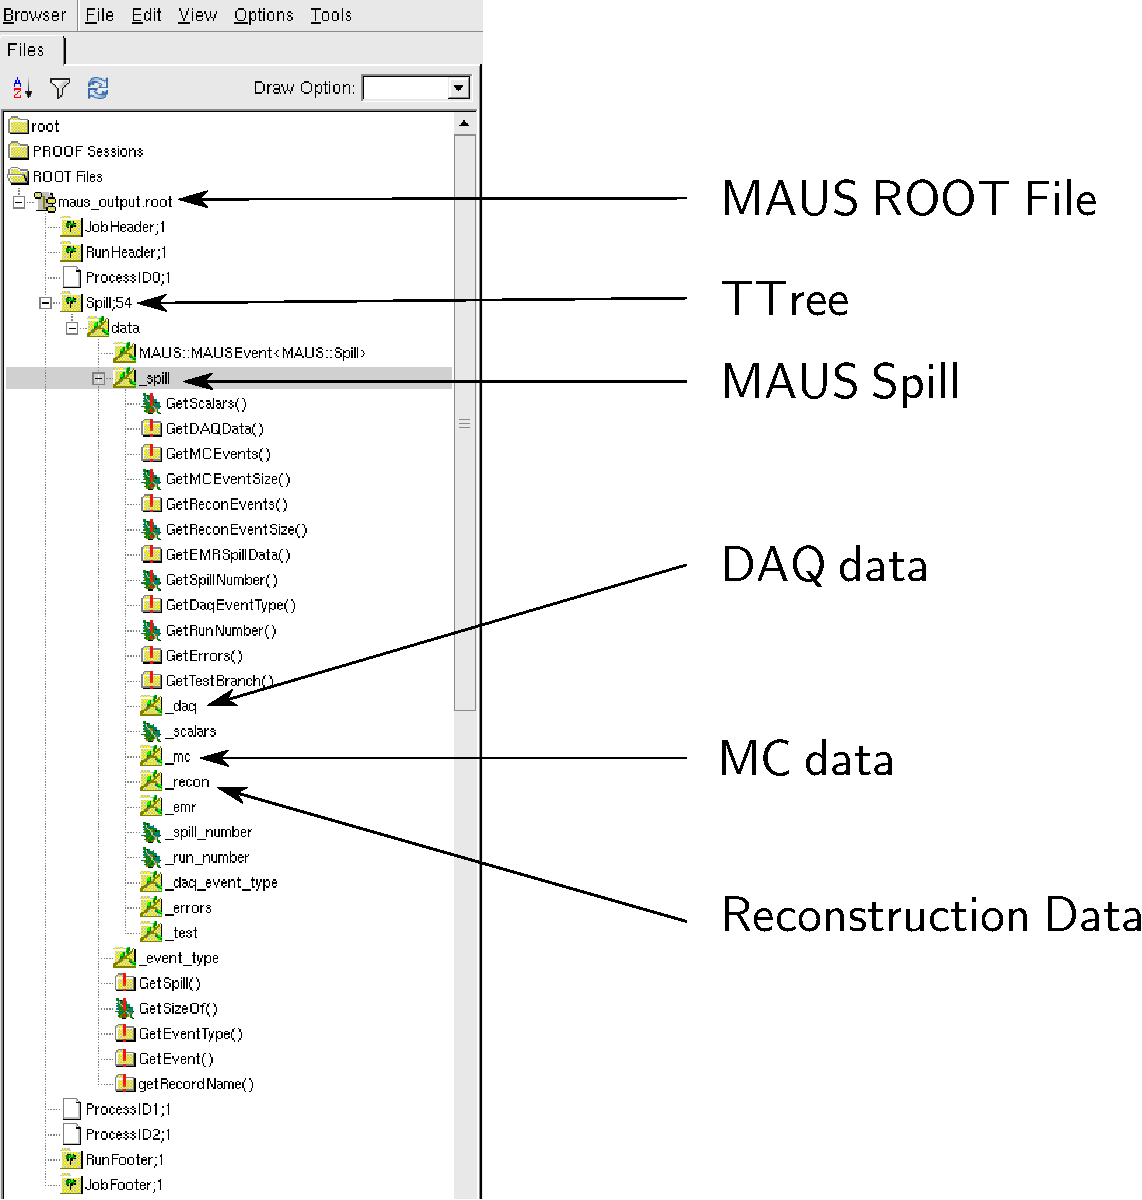
\includegraphics[width=0.5\linewidth]{./graphics/TBrowser.pdf}
      \caption{The top few levels of a MAUS ROOT file, as shown by a ROOT TBrowser.}
      \label{fig:TBrowser}
    \end{center}
  \end{figure}

  There are three standard ways of accessing the data stored in the ROOT file: via ROOT directly (either manually through the ROOT interpretter or with an interpretted ROOT script); via Python using PyROOT (again either through the Python interpretter directly or with a Python script); or with a C++ programme using the ROOT libraries.  All three methods require the MAUS data structure library to be loaded to interpret the data (described in the sections below).

  Both the ROOT and Python methods allow the data inside the TTree to be accessed either directly from the TTree (using ``\texttt{tree->Draw(...)}''), or loaded back into data structure classes in memory.  C++ can only use the latter.  Direct plotting from a the TTree allows for quick and easy browsing of data, whereas loading data back into data structure classes allows greater versatility in analysis.

  It is important to note that \textit{ROOT allows direct plotting from a TTree only down to a few levels of nested data} - hence data nested too deeply into the MAUS data structure cannot be plotted directly from the Spill TTree, either by the ROOT or Python interpretter. In order to plot such data, the data from each spill must be loaded back from the TTree into data structure objects in memory. 

  Interactive plotting directly from TTrees is discussed for ROOT in section~\ref{sec:ROOTPlottingDirectlyFromTTree} and for Python in section~\ref{sec:PythonPlottingDirectlyFromTTree}. Loading data back into data structure classes is discussed for ROOT in section~\ref{sec:RootAnalysisDatastructure}, for Python in section~\ref{sec:PythonAnalysisDatastructure} and for C++ in section~\ref{sec:C++Analysis}.

\lstset{style=customcpp}

  \subsection{Analysis with the ROOT interpreter}
  \label{sec:RootAnalysis}

  \subsubsection{Loading Data}
  Source the MAUS environment and load an interactive ROOT session.  From the ROOT command line load the MAUS data structure library:
  \begin{lstlisting}
.L $MAUS_ROOT_DIR/build/libMausCpp.so
  \end{lstlisting}
  Load the ROOT output file produced by MAUS:
  \begin{lstlisting}
TFile f1("maus_output.root")
  \end{lstlisting}

  \subsubsection{ROOT Scripts}
  Commands may be automated with a ROOT script, which is simply a collection of ROOT commands contained between an opening \texttt{\{} and closing \texttt{\}} in a text file. An important difference to note however is that loading the MAUS data structure library follows a slightly different format when in a script compared to using the ROOT interpreter directly.  The library must now be loaded by calling \texttt{gSystem->Load}:
  \begin{lstlisting}
maus_root_dir = TString(gSystem->Getenv("MAUS_ROOT_DIR"));
gSystem->Load(maus_root_dir + "/build/libMausCpp.so");
  \end{lstlisting}

  \subsubsection{Plotting directly from a TTree}
  \label{sec:ROOTPlottingDirectlyFromTTree}
  Once the data structure and MAUS root file have been loaded, data can be explored using a GUI via the ROOT TBrowser:
  \begin{lstlisting}
TBrowser b
  \end{lstlisting}
  A example of using the TBrowser to navigate the data structure and plot a histogram is shown in figure~\ref{fig:NPE}.

  The ROOT command line may also be used to plot data interactively. For example, the histogram shown in figure~\ref{fig:NPE} could be drawn directly using the command:
  \begin{lstlisting}
Spill.Draw("data._spill._recon->_scifi_event->_scifispacepoints._npe")
  \end{lstlisting}

  \begin{figure}[hbt]
    \begin{center}
      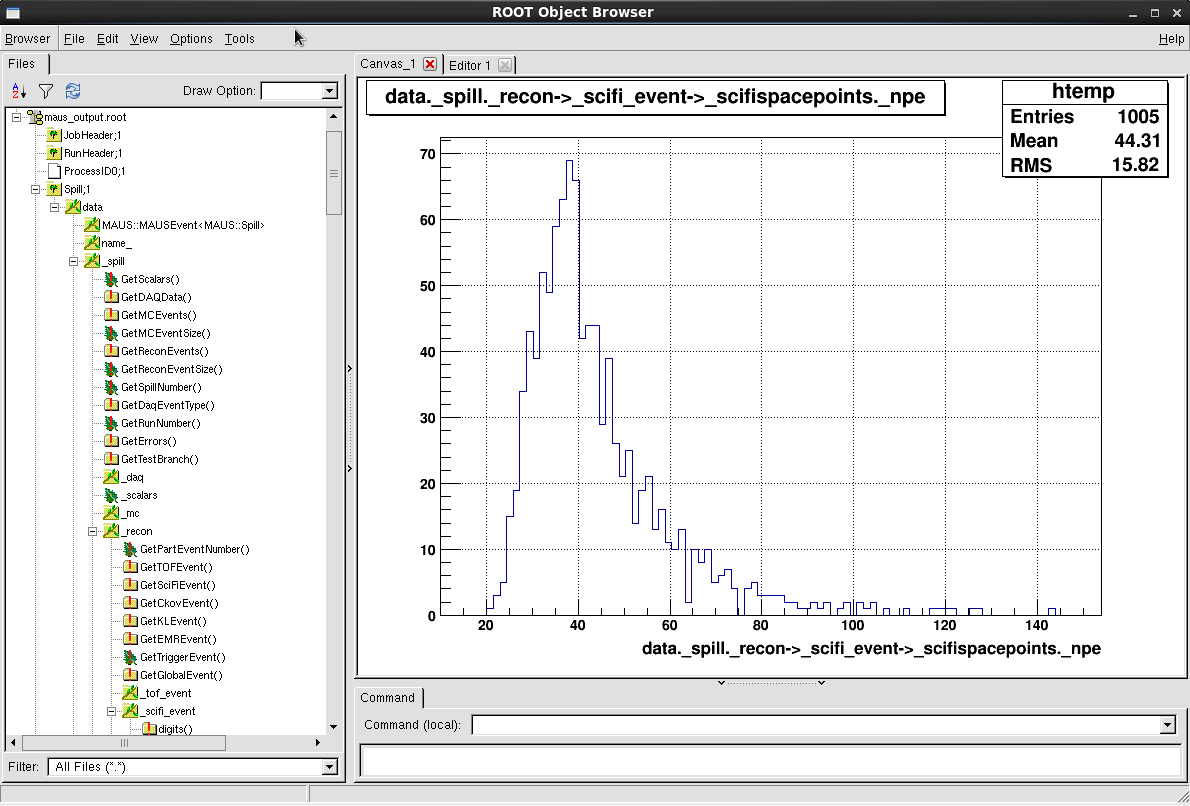
\includegraphics[width=0.8\linewidth]{./graphics/MC-SpacePoint-NPE.png}
      \caption{A ROOT TBrowser plotting the number of photoelectrons in every SciFi SpacePoint for a short MC run.}
      \label{fig:NPE}
    \end{center}
  \end{figure}

  \subsubsection{Reloading the Datastructure}
  \label{sec:RootAnalysisDatastructure}
  To load data back into MAUS data structure classes from the TTree a MAUS Data object pointer must be assigned to the memory address of the MAUS Data object held by the TTree. All the entries in the TTree can then be looped over which will update the pointer to the next spill's Data object each time.  A short ROOT script example which reproduces the histogram in figure~\ref{fig:NPE} is shown below, and is also available to download from \url{http://micewww.pp.rl.ac.uk/documents/140} as ``root\_analysis\_example.C''.
  \begin{lstlisting}
{
  // Load the MAUS data structure
  maus_root_dir = TString(gSystem->Getenv("MAUS_ROOT_DIR"));
  gSystem->Load(maus_root_dir + "/build/libMausCpp.so");

  // Set up the ROOT file and data pointer
  TFile f1("maus_output.root"); // Load the MAUS output file
  TTree *T = f1.Get("Spill");   // Pull out the TTree
  MAUS::Data *data_ptr; // Variable to store Data from each spill
  // Set address of data_ptr to Data object in TTree
  T->SetBranchAddress("data", &data_ptr);  
  
  // Create the histogram
  TH1D* h1 = new TH1D("npe", "SciFi Spacepoint NPE", 100, 0, 150);
  h1->GetXaxis()->SetTitle("Number of photoelectrons");
  h1->SetLineColor(kBlue);

  // Loop over all spills
  for (size_t i = 0; i < T->GetEntries(); ++i) {
    T->GetEntry(i);  // Update the spill pointed to by data_ptr
    MAUS::Spill* spill = data_ptr->GetSpill();  // Get the spill
    if (spill == NULL ||
        !(spill->GetDaqEventType() == "physics_event")) continue;
    std::cout << "Spill: " << spill->GetSpillNumber() << "\n";
    std::vector<MAUS::ReconEvent*>* revts = spill->GetReconEvents();
    // Loop over recon events in spill
    for ( size_t j = 0; j < revts->size(); ++j ) {
      if ( !revts->at(j) ) continue; // Check event pointer
      MAUS::SciFiEvent* sfevt = revts->at(j)->GetSciFiEvent();
      std::vector<SciFiSpacePoint*> spnts = sfevt->spacepoints();
      // Loop over spacepoints
      for ( size_t k = 0; k < spnts.size(); ++k ) {
        h1->Fill(spnts[k]->get_npe()); // Fill histo with npe
      }
    }
  }
  // Draw the histogram
  TCanvas * c1 = new TCanvas("c1", "SF Spacepoint NPE", 900, 600);
  h1->Draw();
}
  \end{lstlisting}
  
  \subsection{Analysis with Python}
  \label{sec:PythonAnalysis}

  \subsubsection{Loading Data}
  Source the MAUS environment and load an interactive Python session.  From the Python interpreter load ROOT and the MAUS data structure library:
  \begin{lstlisting}
>>> import libMausCpp
>>> from ROOT import *
  \end{lstlisting}
  MAUS data structure classes are now accessible.  For example, to create a Spill object:
  \begin{lstlisting}
>>> spill = MAUS.Spill()
  \end{lstlisting}
  \textbf{NB}: Remember to add the trailing ``\texttt{()}'' or the class contructor will not be called.

  A MAUS output file may now be loaded:
  \begin{lstlisting}
>>> f1 = TFile("maus_output.root")
  \end{lstlisting}

  \subsubsection{Plotting directly from a TTree}
  \label{sec:PythonPlottingDirectlyFromTTree}
  Once ROOT and the MAUS data structure are loaded, all the tools available in ROOT are available from Python.  For example, to load a TBrowser use:
  \begin{lstlisting}
>>> b = TBrowser()
  \end{lstlisting}
  To reproduce the histogram in simply use
  \begin{lstlisting}
>>> Spill.Draw("data._spill._recon->_scifi_event->_scifispacepoints._npe")
  \end{lstlisting}

  \subsubsection{Reloading the Datastructure}
  \label{sec:PythonAnalysisDatastructure}
  The same principles used in the ROOT case apply to reloading data in to the MAUS data structure classes from the TTree.  An example script which reproduces the histogram in figure~\ref{fig:NPE} is shown below, and is also available to download from \url{http://micewww.pp.rl.ac.uk/documents/140} as ``python\_analysis\_example.py''.

\lstset{style=custompy}

  \begin{lstlisting}
#!/usr/bin/env python

import libMausCpp
from ROOT import *

# Set up the ROOT file and data pointer
f1 = TFile("maus_output.root")
t1 = f1.Get("Spill")
data_ptr = MAUS.Data()
t1.SetBranchAddress("data", data_ptr)

# Create the histogram
h1 = TH1D("h1", "Spacepoint NPE", 100, 0, 150);
h1.GetXaxis().SetTitle("Number of photoelectrons")
h1.SetLineColor(kBlue)

# Loop over all spills
for i in range(1, t1.GetEntries()):
    t1.GetEntry(i) # Update the spill pointed to by data_ptr
    spill = data_ptr.GetSpill()
    if spill.GetDaqEventType() == "physics_event":
        # Loop over recon events in spill
        for j in range(spill.GetReconEvents().size()):
            sfevt = spill.GetReconEvents()[j].GetSciFiEvent()
            # Loop over spacepoints
            for k in range(sfevt.spacepoints().size()):
                spoint = sfevt.spacepoints()[k]
                h1.Fill(spoint.get_npe())

# Draw the histogram
c1 = TCanvas("c1", "SF Spacepoint NPE", 900, 600)
h1.Draw()
raw_input("Press Enter to finish...")
  \end{lstlisting}

  \subsubsection{ROOT alternatives}
  Once the MAUS data structure has been repopulate from the TTree as described above, alternative tools may be used to produce the desired histograms, plots, etc.  MAUS comes bundled with the popular Python \textit{numpy} and \textit{matplotlib} packages, which are ready to use in the Python interpretter.
  
  \subsection{Analysis with C++}
  \label{sec:C++Analysis}
  The fastest method for large scale data analysis is to compile a C++ programme which calls on the ROOT and MAUS data structure headers and libraries.  The programme structure is very close to that of the ROOT script described in section~\ref{sec:RootAnalysisDatastructure}. An important difference to note is that instead of loading the MAUS output ROOT file directly, a custom C++ streamer class, \textit{irstream} may be used, which serialises the TFile data ready for use.  

  An example source file which recreates the histogram in figure~\ref{fig:TBrowser} is produced below, and is also available to download from \url{http://micewww.pp.rl.ac.uk/documents/140} as ``cpp\_analysis\_example.cc''. It produces an executable which takes the MAUS output ROOT file an argument and will display the histogram to screen.  NB: In order to display the histogram while the application is running, the ROOT class ``TApplication'' must be used. If the purpose of the application was just to save the output to, say, a graphics file, this would not be needed.

\lstset{style=customcpp}

  \begin{lstlisting}  
#include <iostream>
#include <string>
#include <vector>

#include "TCanvas.h"
#include "TH1D.h"
#include "TApplication.h"

#include "src/common_cpp/JsonCppStreamer/IRStream.hh"
#include "src/common_cpp/DataStructure/Spill.hh"
#include "src/common_cpp/DataStructure/Data.hh"
#include "src/common_cpp/DataStructure/ReconEvent.hh"
#include "src/common_cpp/DataStructure/SciFiEvent.hh"
#include "src/common_cpp/DataStructure/SciFiSpacePoint.hh"

/** Access Tracker data using ROOT */

int main(int argc, char *argv[]) {
  // First argument to code should be the input ROOT file name
  std::string filename = std::string(argv[1]);

  // Set up ROOT app, input file, and MAUS data class
  TApplication theApp("App", &argc, argv);
  std::cout << "Opening file " << filename << std::endl;
  irstream infile(filename.c_str(), "Spill");
  MAUS::Data data;

  // Create the histogram
  TH1D* h1 = new TH1D("npe", "SciFi Spacepoint NPE", 100, 0, 150);
  h1->GetXaxis()->SetTitle("Number of photoelectrons");
  h1->SetLineColor(kBlue);

  // Loop over all spills
  while ( infile >> readEvent != NULL ) {
    infile >> branchName("data") >> data;
    MAUS::Spill* spill = data.GetSpill();
    if (spill == NULL || spill->GetDaqEventType() != "physics_event")
      continue;
    std::cout << "Spill: " << spill->GetSpillNumber() << "\n";
    std::vector<MAUS::ReconEvent*>* revts = spill->GetReconEvents();

    // Loop over recon events in spill
    for ( size_t i = 0; i < revts->size(); ++i ) {
      if ( !revts->at(i) ) continue;
      MAUS::SciFiEvent* sfevt = revts->at(i)->GetSciFiEvent();

      // Loop over spacepoints
      std::vector<MAUS::SciFiSpacePoint*> spnts = sfevt->spacepoints();
      std::vector<MAUS::SciFiSpacePoint*>::iterator spnt;
      for ( spnt = spnts.begin(); spnt != spnts.end(); ++spnt ) {
        h1->Fill((*spnt)->get_npe());
      }
    } // ~Loop over Recon events
  } // ~Loop over all spills

  // Draw the histogram
  TCanvas * c1 = new TCanvas("c1", "SF Spacepoint NPE", 900, 600);
  c1->cd();
  h1->Draw();
  theApp.Run();
}
  \end{lstlisting}

Due to the considerable number of dependencies, it is easier to use a build system to compile this, rather than running the compiler directly.  Below is an example Makefile which can be used to compile and link the above the example (assuming a source file of ``cpp\_analysis\_example.cc''.). It is also available to download from \url{http://micewww.pp.rl.ac.uk/documents/140} as ``Makefile''.

\newpage

\lstset{style=custommake}

\begin{lstlisting}
CC = g++
CFLAGS = -DDEBUG -ggdb -Wall

all : cpp_analysis_example

cpp_analysis_example : cpp_analysis_example.cc
  $(CC) $(CFLAGS) cpp_analysis_example.cc -o cpp_analysis_example \
                        -I${MAUS_ROOT_DIR}/ \
                        -I${MAUS_ROOT_DIR}/src/common_cpp \
                        -I${MAUS_ROOT_DIR}/src/legacy \
                        -I${MAUS_THIRD_PARTY}/third_party/install/include \
                        -I${ROOTSYS}/include \
                        -L${MAUS_ROOT_DIR}/build/ \
                        `root-config --ldflags` \
                        `${ROOTSYS}/bin/root-config --glibs` \
                        -lMausCpp \
                         -Wl,--no-as-needed

clean:
  rm cpp_analysis_example
\end{lstlisting}

\section{Event Viewer}

MAUS comes bundled with a number of applications for visualising events. Two shall be described here: EVSimpleExporter and EventViewer. EVSimpleExporter is used to process MAUS output files and produce heprep files which visualises both the detector geometry and reconstructed particle tracks and hits. EventViewer is a Qt-based application which visualises reconstructed tracks and hits without the detectors. Both applications share common code and are not built by default in MAUS.

\subsection{Building the Event Viewer Package}
The dependencies for the event viewer package are as follows:

\begin{itemize}
 \item MAUS version $\ge$ 2.4.0
 \item Qt (for EventViewer)
 \item Java runtime (for the HepRApp viewer)
\end{itemize}

The package may be built as follows:
\begin{itemize}
 \item Navigate to the MAUS root directory and source env.sh
 \item Navigate to \texttt{src/utilities/event-viewer}
 \item Run \texttt{build.sh}
\end{itemize}

More details are available in the package README. This should produce two executables, EVSimpleExporter and EventViewer.

\subsection{The Qt Event Viewer}
Run the EventViewer executable. Use the elipsis button in the top right of the window to open a file selection box and select the MAUS output root file containing the data to be visualised. Wait while the application scans the file (progress can monitored on the command prompt). Once the file has finished loading different events and spills may be navigated and visualised using the buttons found in the bottom left of the window, or using the number entry boxes in the bottom right. 

Different data views are present in the form of tabs immediately above the plotting area. Currently '``Position'', ``Momentum'' and ``Tracker Clusters'' views are implemented. The plots may be panned and zoomed using the mouse. Data from different detectors may switched on or off using the tick boxes at the bottom of the screen.

A screenshot of the EventViewer is shown in figure~\ref{fig:QtEventViewer}.

\begin{figure}[hbt]
  \begin{center}
    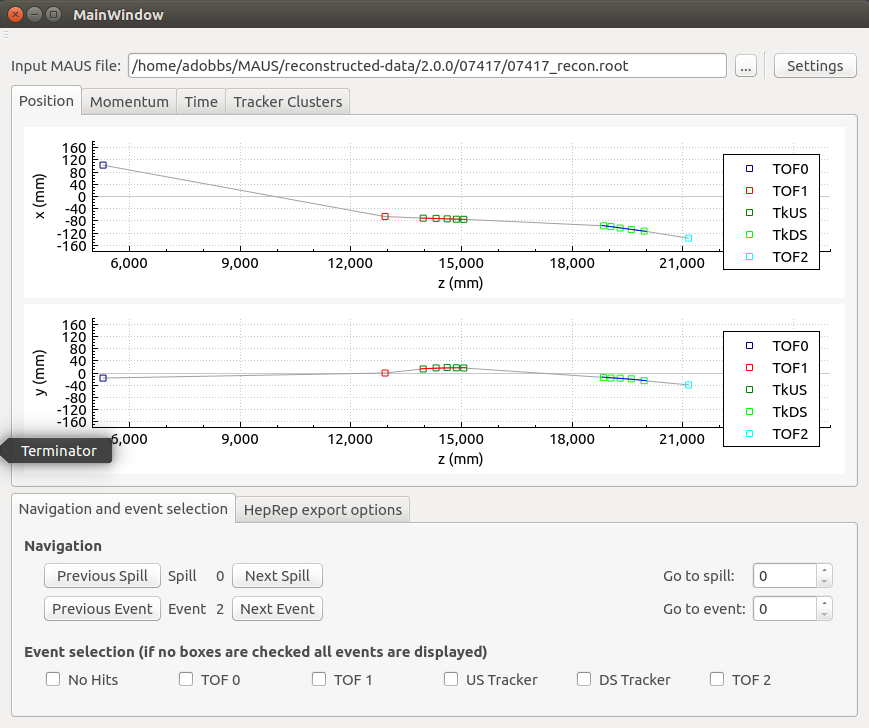
\includegraphics[width=0.8\linewidth]{./graphics/QtEventViewer.png}
    \caption{The Qt Event Viewer Application}
    \label{fig:QtEventViewer}
  \end{center}
\end{figure}

\subsection{The EVSimpleExporter}
The EVSimpleExporter creates heprep files from MAUS output files (other formats may be added in the future). Run the executable with a \texttt{-h} flag to display the different command line options. Spills 0 to 10 from the MAUS output file ``maus\_output.root'' may be output to heprep file using the following command:

 \begin{lstlisting}
  ./EVSimpleExporter -f maus_output.root -sr 0 10
 \end{lstlisting}

The heprep files will by default be created in the current working directory, but this may be altered by setting the \texttt{EV\_DEST\_DIR} environment variable to a different directory. It advisable not to store the output heprep files in the event viewer source directory as one of the source files (``MICEGeometryMinimal.heprep'', describing the geometry) has a ``.heprep'' extension and so may get deleted accidently during clean ups. 

The heprep files may be visualised using the HepRApp application (located in \texttt{third\_party/install/} \texttt{heprep}). For example:

\begin{lstlisting}
 java -jar ${MAUS_THIRD_PARTY}/third_party/install/heprep/HepRApp.jar MICEEvent_7417_9_0.heprep
\end{lstlisting}

Loading the HepRApp application from the event-viewer source directory will allow the application to find a custom settings file (``user.properties'') which will load useful views into the viewer automatically.

A screenshot showing the HepRApp viewer output is shown in figure~\ref{fig:HepRApp}.

\begin{figure}[hbt]
  \begin{center}
    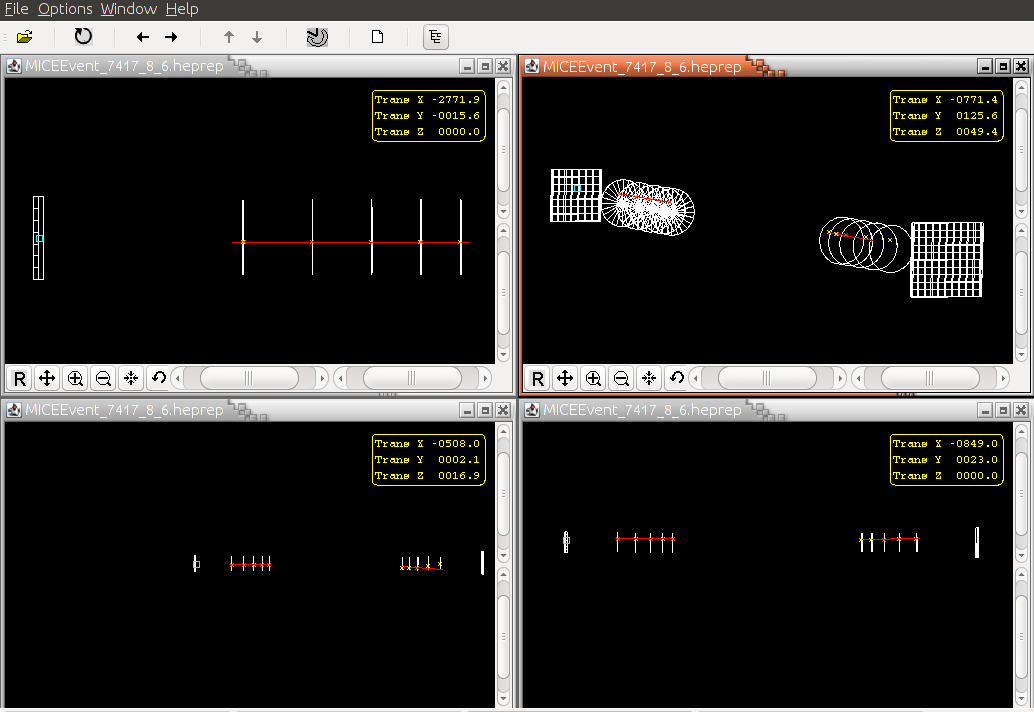
\includegraphics[width=1.0\linewidth]{./graphics/HepRApp.png}
    \caption{The HepRApp viewer, visualising a file produced by EVSimpleExporter.}
    \label{fig:HepRApp}
  \end{center}
\end{figure}




\appendix

\section{Module Descriptions}
\label{ModuleDescriptions}
  \subsection{Input}
    \begin{small}
    \noindent
      \renewcommand{\arraystretch}{1.5}
      \begin{tabular}{| l | l |}
        \hline
        \textbf{Module} & \textbf{Description} \\
        \hline
        InputCppDAQOfflineData & Unpack real data offline \\
        InputCppDAQOnlineData & Used for online reconstruction \\
        InputCppRoot & Read in data from a ROOT file \\
        InputPyJSON & Read in data from a JSON file \\
        InputPySpillGenerator & Make a spill structure for simulation \\
        \hline
      \end{tabular}
      \renewcommand{\arraystretch}{1.0}
    \end{small}
    
  \subsection{Output}
    \begin{small}
    \noindent
      \renewcommand{\arraystretch}{1.5}
      \begin{tabular}{| l | l |}
        \hline
        \textbf{Module} & \textbf{Description} \\
        \hline
        OutputCppRoot & Output data to a ROOT file \\
        OutputPyImage & Output data as an image file \\
        OutputPyJSON & Output data as a JSON file \\
        \hline
      \end{tabular}
      \renewcommand{\arraystretch}{1.0}
    \end{small}

  \newgeometry{left=2cm,right=2cm}
  \subsection{Map}
    \begin{small}
    \noindent
      \renewcommand{\arraystretch}{1.5}
      \begin{tabular}{| l | l | l |}
        \hline
        \textbf{Module} & \textbf{Precursor} & \textbf{Description} \\
        \hline
        MapCppEMRMCDigitization & MapPyMCReconSetup & Digitise EMR MC data \\
        MapCppEMRPlaneHits & MapPyMCReconSetup & Create EMR bar hits \\
        MapCppEMRRecon & MapCppEMRPlaneHits & Reconstruct the EMR data \\
        MapCppGlobalPID & MapCppGlobalTrackMatching & Perform PID using Global data \\
        MapCppGlobalReconImport & Detector maps & Import detector info to Global tracking \\
        MapCppGlobalTrackMatching & MapCppGlobalReconImport & Reconstruct Global tracks \\
        MapCppKLCellHits & MapCppKLDigits OR & Construct hits in the KL \\
         & MapCppKLMCDigitizer & \\
        MapCppKLDigits & MapPyReconSetup & Produce KL digits from real data \\
        MapCppKLMCDigitizer & MapPyMCReconSetup & Produce KL digits from MC data \\
        MapCppSimulation & MapPyBeamMaker OR & GEANT4 sim of beam through MICE \\
         & MapPyBeamlineSimulation & \\
        MapCppTOFDigits & MapPyReconSetup & Produce TOF digits from real data \\
        MapCppTOFMCDigitizer & MapPyMCReconSetup & Produce TOF digits from MC data \\
        MapCppTOFSlabHits & MapCppTOFDigits OR & Reconstruct TOF slab hits \\
         & MapCppTOFMCDigitizer & \\
        MapCppTOFSpacePoints & MapCppTOFSlabHits & Reconstruct TOF spacepoints \\
        MapCppTrackerDigits & MapPyReconSetup & Produce Tracker digits from real data \\
        MapCppTrackerMCDigitization & MapPyMCReconSetup & Produce Tracker digits from MC data \\
        MapCppTrackerMCNoise & MapCppSimulation & Add noise to the Tracker simulation \\
        MapCppTrackerRecon & MapCppTrackerDigits OR & Reconstruct the Tracker data \\
         & MapCppTrackerMCDigitization & \\
        MapPyBeamlineSimulation & InputPySpillGenerator & Generate beam with G4BeamLine \\
        MapPyBeamMaker & InputPySpillGenerator & Generate beam with GEANT4 \\
        MapPyCkov & MapPyMCReconSetup & Reconstruct the CKOV data \\
        MapPyDoNothing & None & No maps \\
        MapPyGroup & None & Used to add multiple maps \\
        MapPyMCReconSetup & MapCppSimulation & Setup for MC reconstrucuted data \\
        MapPyReconSetup & InputCppDAQOfflineData OR & Setup for real reconstrucuted data \\
         & InputCppDAQOnlineData & \\
        MapPyScalersDump & InputCppDAQOfflineData OR & Print scaler data \\
         & InputCppDAQOnlineData & \\
        \hline
      \end{tabular}
      \renewcommand{\arraystretch}{1.0}
    \end{small}
    \restoregeometry

\pagebreak

  \subsection{Reduce}
    \begin{small}
    \noindent
      \renewcommand{\arraystretch}{1.5}
      \begin{tabular}{| l | l |}
        \hline
        \textbf{Module} & \textbf{Description} \\
        \hline
        ReduceCppPatternRecognition & Display tracker pattern recognition tracks \\
        ReducePyCkovPlot & Display CKOV data \\
        ReducePyDoNothing & No reducer \\
        ReducePyKLPlot & Display data \\
        ReducePyTOFPlot & Display TOF data \\
        \hline
      \end{tabular}
      \renewcommand{\arraystretch}{1.0}
    \end{small}


\section{Common Parameters and their Defaults}
\label{sec:CommonParameters}

All the MAUS parameters and their defaults values can be found in:

\vspace{0.5cm}

\texttt{src/common\_py/ConfigurationDefaults.py}

\vspace{0.5cm}

\noindent
A table of some common parameters is produced below.
\vspace{0.5cm}

\begin{small}
\noindent
  \renewcommand{\arraystretch}{1.5}
  \begin{tabular}{| l | l | l |}
    \hline
    \textbf{Parameter} & \textbf{Default}& \textbf{Description}  \\
    \hline
    daq\_data\_file & '05466.001' & The real data file \\
    daq\_data\_path & 'src/input/InputCppDAQData' & Location of real data \\
    input\_root\_file\_name & 'maus\_input.root' & Input ROOT file name  \\
    geometry\_download\_directory & "files/geometry/download" & CDB geometry download directory \\
    output\_root\_file\_name & 'maus\_output.root' & Output ROOT file name  \\
    keep\_only\_muon\_tracks & False & Simulate muon tracks \\
    particle\_decay & True & Should particles decay \\
    physics\_model & "QGSP\_BERT" & Physics package \\
    physics\_processes & "standard" & Physics processes \\
    reconstruction\_geometry\_filename & "" & The simulation geometry \\
     & & (blank $\Rightarrow$ use simulation geometry) \\
    reference\_physics\_processes & "mean\_energy\_loss" & Physics processes of ref. part. \\
    simuation\_geometry\_file & "Test.dat" & The simulation geometry \\
    spill\_generator\_number\_of\_spills & 100 & \# of spills to simulate \\
    verbose\_level & 1 & Amount of screen output \\
    \hline
  \end{tabular}
  \renewcommand{\arraystretch}{1.0}
\end{small}

\section{Navigating the Source Code}

\begin{small}
\noindent
  \renewcommand{\arraystretch}{1.5}
  \begin{tabular}{| l | l |}
    \hline
    \textbf{Description} & \textbf{Location} \\
    \hline
    Executables & bin, bin/user \\
    Documentation & doc \\
    Input modules & src/input \\
    Map modules & src/map \\
    Reduce modules & src/reduce \\
    Output modules & src/output \\
    C++ backend code & src/common\_cpp \\
    Python backend code & src/common\_py \\
    Datastructure & src/common\_cpp/Datastructure \\
    Legacy Geometry & src/legacy/FILES/Models \\
    Tests & tests \\
    Third party libraries & third\_parties \\
    \hline
  \end{tabular}
  \renewcommand{\arraystretch}{1.0}
\end{small}


\section{Useful Information}
\label{sec:UsefulInformation}
  \begin{itemize}
    \item The MICE website: \url{http://mice.iit.edu}
    \item The MAUS wiki: \url{http://micewww.pp.rl.ac.uk/projects/maus/wiki}
    \item Download MAUS: \url{http://micewww.pp.rl.ac.uk/maus/}
    \item The MICE offrec processed datastore: \url{http://reco.mice.rl.ac.uk/}
    \item The GRID MICE datastore: \url{http://www.hep.ph.ic.ac.uk/micedata/}
    \item The MICE CDB viewer: \url{http://cdb.mice.rl.ac.uk/cdbviewer/}
    \item Example analysis code: \url{http://micewww.pp.rl.ac.uk/documents/140}
  \end{itemize}


\end{document}
